\section{Introduction}
% --- Teaser figure ---------------------------------------------------
% Placed directly below the author block and above the abstract, as in
% the original submission. Edit the caption/label below.
\begin{figure}[t]
\centering
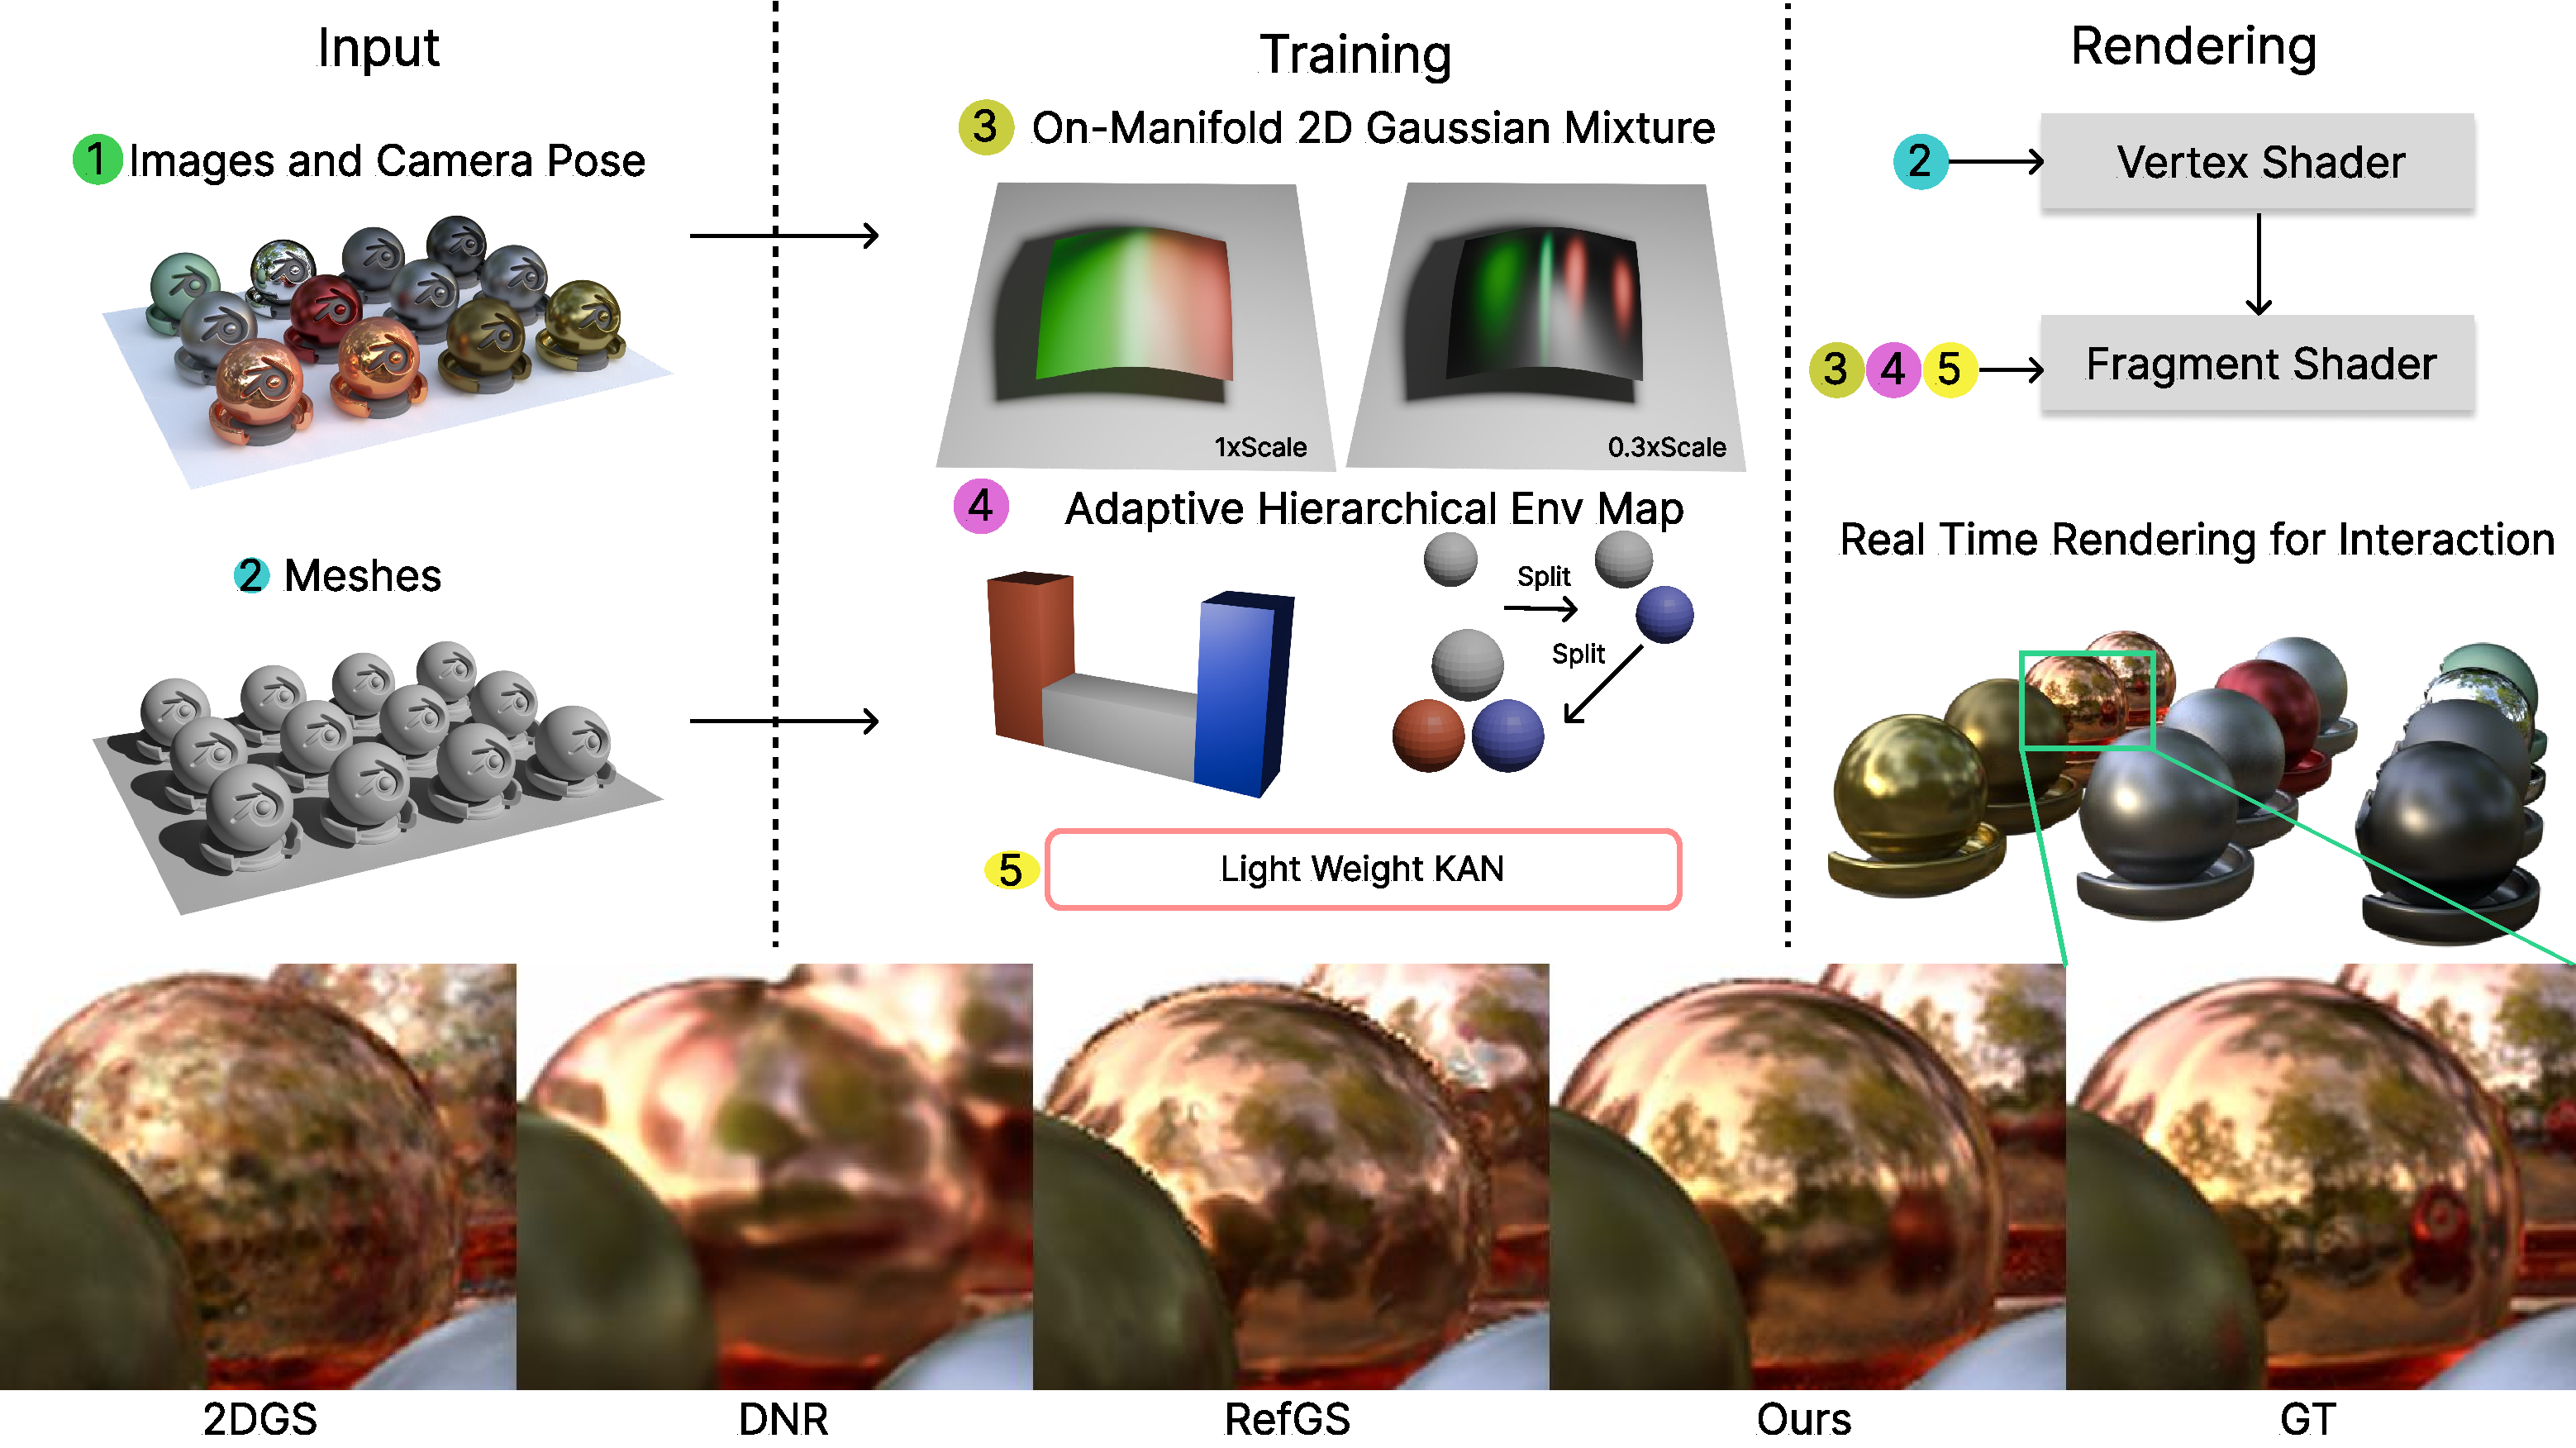
\includegraphics[width=\linewidth]{figs/tiser.pdf}
\caption{%
\textbf{Automatic Neural Baking bakes highly reflective, view-dependent appearance directly onto a mesh, rendering it in real time (>60 FPS) with fidelity that surpasses state-of-the-art flexible-mesh methods.}
\emph{Comparison}: on Shiny-Blender, our method reproduces sharp, high-frequency specular reflections that 2DGS~\citep{2DGS} and DNR~\citep{DNR} smears and that RefGS~\citep{refgs} recovers less crisply, while running natively in a standard rasterizer rather than requiring depth-sorted splat rendering.
\emph{Pipeline}: from posed reference images ~\badgeimg{} and the corresponding triangle mesh~\badgemesh, we optimize three interchangeable, rasterizer-native modules - an on-manifold 2D Gaussian mixture storing diffuse albedo and reflectivity~\badgegmm, an adaptive, hierarchical environment map capturing self-reflection ~\badgeenv; and a lightweight KAN that evaluating the reflection equation for far-field specular~\badgekan - all evaluated per-fragment in a standard fragment shader
\badgemesh\,\badgegmm\,\badgeenv\,\badgekan.%
}
\label{fig:teaser}
\end{figure}
% ----------------------------------------------------------------------

Interactive applications such as games, virtual reality, and other online rendering, demand photorealistic imagery in real time (typically $\geq 60$~FPS).
The standard baking-and-rasterization pipeline meets this by precomputing appearance offline into textures over the mesh, which a fragment shader then samples cheaply at run time~\citep{RealTimeRendering}.


Automating this stage, however, remains hard for the shiny, view-dependent materials that matter most:
the usual baked formats, for instance, lightmaps or low-order Spherical Harmonic (SH) probes, store only smooth, view-independent lighting and miss angle-dependent highlights~\citep{AllFrequency, curveSurfaces, nerfTexture}.
Baking also presupposes a global UV atlas, whose automatic construction remains fragmented and largely manual~\citep{Levy2002LSCM, poranne2017autocuts, li2018optcuts, srinivasan2024nuvo}. Per-face texturing such as Ptex~\citep{ptex} removes the UV atlas, but as a static texture it still cannot capture high-frequency, view-dependent reflection.
The seminal automatic neural baking method is Deferred Neural Rendering (DNR)~\citep{DNR}, which bakes learned neural textures onto a mesh and decodes them at render time.
However, DNR shares the same weakness as classical baking and cannot reproduce high frequency view-dependent color.
Our method is a direct, modern successor to it: The mesh is an input, not an output; in our setting it is an artist-authored asset, the standard target of baking workflows. Like DNR, it is a traditional baking method that produces a baked mesh asset. Unlike DNR, it also captures the sharp, view-dependent appearance that baking has always lacked. 

Such appearance has instead been the domain of neural and splat representations. Neural Radiance
Fields (NeRFs)~\citep{NeRFVanilla} and 3D Gaussian Splatting (3DGS)~\citep{3DGS} have
revolutionized novel view synthesis, reaching a photorealism that classical baking cannot match by
treating the scene as a continuous optimization problem.
But they place appearance in the \emph{ambient space}: a continuous field over $\mathbb{R}^3$ for
NeRF, a mixture of anisotropic kernels for 3DGS.
The baking pipeline instead treats an object as a \emph{surface}, a two-dimensional manifold
$\mathcal{M}\subset\mathbb{R}^3$ carrying appearance as a field on $\mathcal{M}$ itself.
Because the ambient field for NeRF and 3DGS has no 2D domain, there is nothing to bake.

Attempts to close this gap do not change the domain. Extraction methods recover a mesh after the
fact~\citep{sugar, gaussianSurfels} but only approximate a surface the representation never carried,
and the primitives themselves remain free in $\mathbb{R}^3$.
2DGS~\citep{2DGS} flattens each ellipsoid into a disk, collapsing the kernel across its normal
direction; this removes thickness, but a sum of such disks scattered through space is still an
ambient-space distribution.
The natural remaining step is to bind the primitives directly to the faces of a known mesh. This is
where the difficulty becomes concrete.

Once primitives are strictly coplanar, their depth keys tie and alpha compositing has no
well-defined order. The standard remedies fail in instructive ways.
Offsetting disk $i$ along the face normal by $\varepsilon_i$ separates two disks by
$(\varepsilon_i-\varepsilon_j)(\mathbf{n}\cdot\mathbf{v})$, where n is the normal of that face, and v is the viewing direction. 
The order changes at grazing angles: small
offsets reproduce the tie, while large ones yield an ordering that flips as the camera orbits, so
gradients from different views disagree about which primitive owns a fragment.
Large offsets also let the optimizer reintroduce extent along $\mathbf{n}$, reinstating the ambient
drift the binding was meant to remove and degrading the surface it is bound to.
Breaking ties by a fixed primitive index is view-stable but imposes an occlusion relation
uncorrelated with geometry.
The obstruction is not depth but \emph{order-dependence itself}: on a single opaque surface no
ordering is both view-stable and geometrically meaningful.


We therefore drop ordering altogether. We bake appearance as an \emph{element-wise field whose
domain is the surface}: a mixture of two-dimensional Gaussian disks anchored to mesh faces in
barycentric coordinates, blended at each fragment by a normalized partition of unity over the $K$
nearest disks. Because the blend is a convex combination rather than an alpha composite, it is
invariant to order; the global $O(N\log N)$ sort becomes an $O(K)$ local gather, with no degeneracy
to avoid. This is a texture in a sense that a neural raster atlas~\citep{DNR} is not: its elements
are individually addressable, movable, mergeable, and differentiable, and it needs no UV atlas. To
our knowledge it is the first differentiable element-wise appearance field defined on the manifold
itself.

On this field we place two modules supplying the view-dependent term: an adaptive hierarchical
environment map that splits the object into near-convex parts, so self-reflection reduces to a local
lookup rather than a secondary ray; and a compact FastKAN decoder~\citep{fastkan, kan} that
interpolates the reflection from sparse views. All three modules are interchangeable, and each is
evaluated per fragment against a single opaque surface. The representation is read and written like
a texture: we demonstrate it in nvdiffrast at over 60 FPS.



The appearance at each surface point is thus a local diffuse color plus a single gated reflection
covering both far-field and near-field (self-)reflection, composited in logit space.
On Shiny-Blender this reaches $36.99$\,dB PSNR; starting instead from an imperfect reconstructed
mesh, optimizing appearance alone also improves that mesh's normal error and Chamfer distance on
every scene.

Our central contribution is the representation; the remaining items are properties it makes
possible.
\begin{itemize}
\item \textbf{An element-wise texture on a 2-manifold.} A differentiable appearance field whose
domain is the mesh surface and whose blending is order-independent, requiring no UV atlas and no
depth sort: an $O(K)$ per-fragment gather replaces the global $O(N\log N)$ sort. We diagnose why
face-bound splats cannot achieve this and measure each failure mode (Sec.~\ref{sec:ablation}).
The surface kernel is interchangeable; we adopt a 2D Gaussian mixture as a strong default
(Sec.~\ref{sec:gmm}).
\item \textbf{Sharp view-dependent appearance, baked.} A FastKAN decoder over an adaptive
hierarchical environment map captures high-frequency specularity, and near-convex decomposition
reduces self-reflection to a local lookup rather than a secondary ray. On Shiny-Blender we reach
$36.99$\,dB PSNR, the best reported result given the same geometry.
\item \textbf{Refining the mesh through appearance alone.} The anchoring that makes the field a
surface parameterization also makes its gradient blind along the surface normal: a disk can ask the
mesh to slide, never to move in or out. We recover that direction by momentarily reading each disk's
gradient in the ambient space the anchoring excludes, then pulling it back onto the vertices through
the same barycentric weights that reconstructed the disk. In this way, the mesh moves while the appearance
field stays a parameterization of it. Starting from a reconstructed mesh~\citep{refgs}, this
improves normal MAE$^\circ$, Chamfer distance, and F1 on all six Shiny-Blender scenes.
\item \textbf{Evaluable in a fragment shader.} Every module is a local, per-fragment operation over
a single opaque surface  without global state, and secondary rays. The representation is therefore
shader-implementable by construction; we realize it in nvdiffrast and render both datasets at over
$60$ FPS.
\end{itemize}